\documentclass{natureprintstyle}
%\documentclass{nature}
\bibliographystyle{naturemag}
\usepackage{epsfig,caption}
\usepackage{color}
\usepackage{bm}
\usepackage{graphicx}
\usepackage{longtable}
\usepackage{amssymb}
\usepackage{rotating}
\usepackage{latexsym}
\usepackage{hyperref}
\usepackage{float}

%\usepackage[switch]{lineno}
%\linenumbers

%%%%%%%%%%%%%%%%%%%%%%%%%%%%%%%%%%%%%%%%%%%%%%%%%%%%%%%%%%%%%%%%%%%
% comment for selecting the best figures to go on web for:
%@arxiver{jvds_sami_vsigma_ellip_LOESS_Age_paper.pdf,jvds_sami_vsigma_ellip_LOESS_Age_transform_paper_resubmit.pdf} 
%%%%%%%%%%%%%%%%%%%%%%%%%%%%%%%%%%%%%%%%%%%%%%%%%%%%%%%%%%%%%%%%%%%

%journal commands
\newcommand{\apj}{Astrophys. J.}
\newcommand{\spie}{Proc. SPIE}
\newcommand{\pasp}{Publ. Astron. Soc. Pac.}
\newcommand{\apjs}{Astrophys. J. Supp.}
\newcommand{\araa}{Annu. Rev. Astron. Astrophys.}
\newcommand{\mnras}{Mon. Not. R. Astron. Soc.}
\newcommand{\apjl}{Astrophys. J. Let.}
\newcommand{\aap}{Astron. Astrophys.}
\newcommand{\aj}{Astron. J.}
\newcommand{\nat}{Nature}
\newcommand{\na}{New Astron. Rev.}
\newcommand{\aaps}{A\&AS}
\newcommand{\procspie}{Proc. SPIE}

%%%%%%%%%%%%%%%%%%%%%%%%%%%%%%%%%%%%%%%%%%%%%%%%%%%%%%%%%%%%%%%%%%%
% my commands

\newcommand{\lcdm}{$\Lambda$CDM}
\newcommand{\hst}{{\it HST}}
\newcommand{\efr}{$R_{\mathrm{eff}}$}
\newcommand{\galfit}{{\sc Galfit}}
\newcommand{\mbh}{$\mathcal M_{\rm BH}$}
\newcommand{\lhost}{$L_{\rm host}$}
\newcommand{\mr}{Mag$_{\rm ~R}$}
\newcommand{\jcap}{Journal of Cosmology and Astroparticle Physics}
\newcommand{\halpha}{${\it H}\alpha$}
\newcommand{\hbeta}{${\it H}\beta$}
\newcommand{\sersic}{S\'ersic}
\newcommand{\lenstronomy}{{\sc Lenstronomy}}
\newcommand{\reff}{{$R_{\mathrm{eff}}$}}
%\newcommand{\kms}{km~s$^{\rm -1}$}
\newcommand{\kms}{\ifmmode{\,\rm{km}\, \rm{s}^{-1}}\else{$\,$km$\,$s$^{-1}$}\fi}
\newcommand{\sigstar}{{$\sigma_*$}}
\newcommand{\mstar}{{$M_*$}}
\newcommand{\Mgii}{Mg$_{\rm II}$}
\newcommand{\Civ}{C$_{\rm IV}$}
\newcommand{\farcs}{\mbox{\ensuremath{.\!\!^{\prime\prime}}}}% fractional arcsecond symbol: 0.''0
%%%%%%%%%%%%%%%%%%%%%%%%%%%%%%%%%%%%%%%%%%%%%%%%%%%%%%%%%%%%%%%%%%%

\title{
%From predictions to observation: scaling relations between supermassive black holes and their host galaxies at $1< z<2$
A successful observational test of black hole and galaxy co-evolution models since $z\sim1.7$
%The first comparison between the observation and simulation of the scaling relations between supermassive black holes and their host galaxies at $1.2< z<1.7$
}
\author{Xuheng Ding$^{1,2}$, 
Tommaso Treu$^{1}$, 
John Silverman$^{3, 4}$,
Aklant K. Bhowmick$^{5}$,
N. Menci$^{6}$,
Tiziana Di Matteo$^{5}$,
et. al.
}

\begin{document}

\maketitle

\let\thefootnote\relax\footnote{
\begin{affiliations}
\item {Department of Physics and Astronomy, University of California, Los Angeles, CA, 90095-1547, USA} 
\item {School of Physics and Technology, Wuhan University, Wuhan 430072, China}
\item {Kavli Institute for the Physics and Mathematics of the Universe (WPI), The University of Tokyo, Kashiwa, Chiba 277-8583, Japan}
\item {Department of Astronomy, School of Science, The University of Tokyo, 7-3-1 Hongo, Bunkyo, Tokyo 113-0033, Japan}
\item{McWilliams Center for Cosmology, Dept. of Physics, Carnegie Mellon University, Pittsburgh PA 15213, USA}
\item{INAF?Osservatorio Astronomico di Roma, via Frascati 33, I-00078 Monteporzio, Italy}
\end{affiliations}
}

\begin{abstract}
Supermassive black holes (BH) harbor at the center of galaxies with their masses correlated to the properties of the host galaxies, including absolute magnitude ($Mag$) and stellar mass (\mstar) known as scaling relations (i.e., \mbh-\lhost, \mbh-\mstar). Observational results have indicated evidence that this correlation evolves with cosmic time, suggesting a scenario that the BH growth predates their host. In theory, positive evolution of BH is also predicted by several simulation projects independently. So far, the simulations have reproduced the relations which have a good agreement to the observational sample from local to intermediate redshift ($0.3<z<1$). It is crucial to extend this study to higher redshift ($z>1$), where the predicted relations are more sensitive to the initial simulating assumptions and any inconsistency could help to pinpoint the incorrect ones.
To this end, we use a sample of 32 X-ray-selected broad-line (type-1) AGNs at $1.2 < z < 1.7$ ($\sim 8.5-10$ billion years ago) to make a direct comparison to the predicted sample from two independent state-of-the-art simulating projects, including MassiveBlack-II (MBII) and semi-analytic models (SAMs). We use \hst\ observed images to study the 32 AGNs in multi-bands and deriving the trustworthy stellar mass measurements and the reliable broad \halpha\ emission lines to estimate the \mbh. Taking the selection bias into account, %by adopting the same selection function to choose the simulating sample,
we find that both models agree well with the data, even though they use very different recipes. These agreements indicate the existence of a causal connection between BH and the host galaxy, which could not be explained by purely a stochastic process. To some extent, our result attests that this connection induces an ordering so that the more massive black holes are linked to the more massive masses. Moreover, we find the intrinsic scatter of our high-$z$ sample is not larger than the simulations and local ones, which is against the central limit theorem. 

\end{abstract}

%\section{Introduction}
The discovery of the correlations between the masses (\mbh) of supermassive black holes (SMBH) and the properties of their host galaxies, such as absolute magnitude ($Mag$) and stellar mass (\mstar), indicates that the growth of BH could be connected to its host galaxy formation. So far, the origin that drives this connection is still unknown, due to the daunting range of scales between the dynamical sphere ($\sim$pc) of the SMBH and their host galaxy ($\sim$10 kpc). A dominant interpretation is so-called AGN feedback, assuming that a small fraction of AGN energy injects to their surrounding gas that regulates the growth of SMBH and its host galaxy. In this scenario, the activity of AGN accretion heats and unbinds significant fractions of the gas and inhibits star formation. Some models have been proposed that the connection between SMBH and its host are connected not in a direct manner but assuming that they share a common gas supply~\cite{Cen2015, Menci2016}. On the other hand, without any physical mechanisms, the statistical convergence from galaxy assembly alone (i.e., dry mergers) may reproduce the observed correlations. In this central limit theorem, a stochastic cloud at high-$z$ (higher scatter) would end up with the scaling relations (lower scatter) as observed today.

To understand this connection, the recent works~\cite{Park15, Tre++07, Bennert11, Woo++08} have analyzed the scaling relations beyond the local redshift {($0.3<z<1$)} with active galactic nuclei (AGN) using {\it Hubble Space Telescope} ({\it HST}) and found an evolution that the growth of SMBHs predated to their host galaxies. However, the observational evidence of evolution at high-$z$ is under debated as it relies on our understanding of systematic uncertainties and selection effects. It has been realized that the improper way to consider the uncertainties and selection effects could result in an {\it apparent} evolution and result in an overestimate of the evolution\cite{Volonteri2011}.

%Why comparison between data and model.
%Summary of recently works.
%The reason to extend to high redshift.
Simulating models are the effective tools that help to understand this connection and rule out the assumptions which could not be satisfied with the observations. In the simulating test, the systematic uncertainties and selection bias would be easy to account for. Recent simulating studies by several projects have made predictions which is in good agreement with the analysis by the observations at intermediate redshift range. For example, the state-of-the-art cosmological hydrodynamical simulations of structure formation (MassiveBlackII) have compared the predicted scaling relations to the \hst\ observation at $0.3<z<1$ and predict a positive evolution that SMBH growth predates the host galaxy~\cite{DeG++15}. Several others works have investigated the scaling relations using large-volume simulations, also well matching the local relation with some redshift evolution, including approaches using the Magneticum Pathfinder SPH Simulations~\cite{Steinborn2015}, the Evolution and Assembly of GaLaxies and their Environments (EAGLE) suite of SPH simulations~\cite{Schaye2015}, and Illustris moving mesh simulation\cite{Sijacki2015, Vogelsberger2014}. Besides hydrodynamic simulations, semi-analytic models~\cite{Menci2014, Menci2016} also have made remarkable progress and recovered the local scaling relations~\cite{Kormendy13}. However, to date, the comparisons to the high-resolution (i.e., \hst) sample were still limited at $z<1$ due to the limitation of the observations.

%A good way to understand this connection is to rely on active galactic nuclei (AGN) and trace the scaling relations to higher redshifts, witnessing how and when does it happen. More recently, there is increasing observational evidence indicating the positive offset exist in the correlation at intermediate redshift range ($0.3<z<1$), implying that galaxies built up around the massive potential wells of mature BHs. Stimulated by the observations, theoretical efforts have been made to include the growth of \mbh\ in the framework of cosmological galaxy formation simulations, and generated the predictions of local scaling relations which match the observations well. Moreover, the simulations predict that the positive offset could be even stronger at redshift range $1<z<2$. 

%Using the samples predicted by the simulation to compare to the observations is beneficial, in particular at high redshift. First, it helps to directly verify the validity of the initial physics prescriptions adopted in the simulation process, and point out the direction where to improve if needed. Second, in turn, the lessons learned in the simulations could be used to investigate the mechanism of the origin of the scaling relation. For example, the feedback originating in the surroundings of BHs, the major merging activities, and the growth of the \mbh\ and the stellar components as connected to the common gas supply have been invoked as the process leading to the co-evolution. Extending the comparison to high redshift help to explore the origin of the evolution directly. Furthermore, adopting the same selection function enable the particular comparison between two equivalent sample, so as to get rid of the systematic bias lead by the selection effects.

% The work that we want to do
	%Sample selection
	%The advantage of our measurements
	%Compare to which simulation? (some introduction)
	%Any expectation?
	%mention the scatter.
To extend, we collected a sample of 32 \hst-observed AGN systems at redshift range $1.2<z<1.7$ from X-ray coverage fields, including COSMOS~\cite{Civano2016}, (E)-CDFS-S~\cite{Lehmer2005, Xue2011}, and SXDS~\cite{Ueda2008}, to compare to the simulating models. The redshift range of our targets is chosen to be high enough ($z>1$) to detect the existence of the evolution offsets and make the comparison to the models, while low enough ($z<2$) to limit the effect of surface brightness dimming. We selected our AGN sample in a well-defined window as in Figure~\ref{fig:AGN_select}, based on the \mbh\ and Eddington ratio. As shown, the \mbh\ are well below the knee of the BH mass distribution to avoid strong selection bias and the Eddington ratio are above the 1\% level to ensure the homogeneity.

We measure reliable \mbh\ and host properties to overcome the systematic. Specifically, the \mbh\ of our sample are estimated using the published near-infrared spectroscopic observations of the broad \halpha\ emission lines, which removes the systematic with \Mgii\ or \Civ. For the inference of properties of the host galaxies, the X-ray selected sample has lower nuclear-to-host ratios at IR band, which facilitates the inference of the host light. We employ the \hst/WFC3 to obtain high-resolution (0\farcs0642 per pixel) imaging data and adopt the state-of-the-art technique to perform the 2-D flux profile decomposition to infer the light of the host galaxy. Moreover, 21/23 systems have \hst/ACS imaging data, which enable us to assess the colors of the host, hence the rest frame R-band magnitude (\mr) and stellar mass (\mstar). 
%We furthermore combining them with the ground-based photometry to carry out the SED fitting, and thus derive the reliable host rest-frame R band luminosity and stellar mass.

\begin{figure}[t]
\includegraphics[width=0.9\linewidth]{AGN_selection.pdf}
\caption{The selection for the 32 AGN sample. The top and right panels are the BH mass function and Eddington ratio function.
}
\label{fig:AGN_select}
\end{figure}

To make the comparison to the simulating models, we adopt two independent simulating projects, including MassiveBlack-II (MBII) and semi-analytic models (SAM). These two models are based on independent model strategies, i.e., hydrodynamic simulation for MBII and semi-analytic model for SAM, respectively. The MassiveBlack-II (MBII) simulation is the highest resolution at the size of a comoving volume $V_{\rm box} = (100~{\rm Mpc}~h^{-1})$, including a self-consistent model for star formation, black hole accretion, and associated feedback. The large simulation volume enables the simulating objects to evolve independently; the high enough mass and spatial resolution meet the requirements for the object details. On the theoretical side, aimed, high-resolution N-body simulations can study specific galaxy systems. However, understanding the mechanism of the scaling relation requires an analytical description of such processes to be implemented into existing semi-analytic models, such as (SAM). 
MBII and SAM have made successful predictions in previous works \cite{Menci2014, Menci2016, Khandai2015}. We refer the interested readers to these works for more details.

%\section*{Results}
%Selection effect into account
We select the AGNs in the MBII simulation at $z=1.5$ and collect their scaling relations to compare with the observed ones. To take the measurement uncertainty and the selection effect into account, we added the random noise to the simulated sample to mimic the scatter effect. The assumed uncertainties are $\Delta$\mbh =0.4~dex, $\Delta$\mr=0.3~dex, $\Delta$\mstar=0.17~dex and $\Delta L_{\rm bol}$=0.03~dex, respectively, which is comparable to the measurement. We then select the sample that falls in the selection window, as shown in Figure~\ref{fig:selectfunc}. We investigated the predicted relations of the \mbh-\mr\ and \mbh-\mstar\ by the MBII and compared to the observational constraints. In Figure~\ref{fig:MBII_comp}, we show the comparisons of both relations and find that the predicted scaling relations have an excellent agreement to the observations. We carry out the linear fitting of the observed sample and the {\it selection-effect-considered} sample using the same slope value. The mismatch of the interceptions between the two lines are relatively small within $1-\sigma$ level. We adopt the {\sc Linmix} to estimate the intrinsic scatter for both sample. Interestingly, the observed sample have an intrinsic scatter of $0.13\pm0.10$~dex, which is not larger than the one in the MBII, which is $0.23\pm0.06$~dex.

\begin{figure}[t]
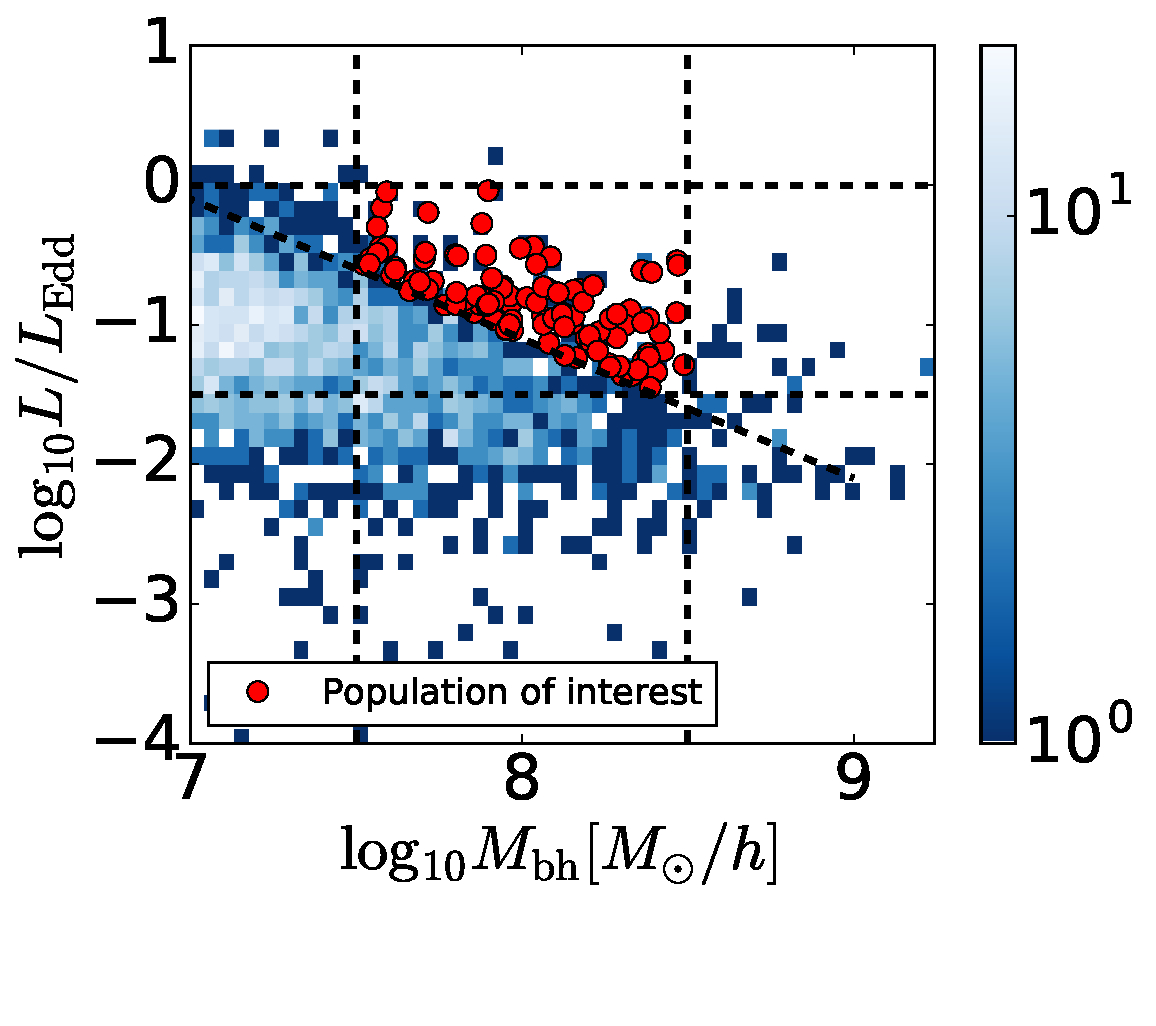
\includegraphics[width=1.0\linewidth]{MBII_selectfunc.pdf}
\caption{The selection window as adopted for selecting the MBII simulated sample. The yellow background clouds shows the overall sample at $z=1.5$. We add the random uncertainty to the simulation and select the ones located in the selection window (i.e. red region). The green sample are the high-$z$ sample.}
\label{fig:selectfunc}
\end{figure}
%comparison to simulation (flux ratio also)

\begin{figure*}[t]%[!b]
\begin{tabular}{c c}
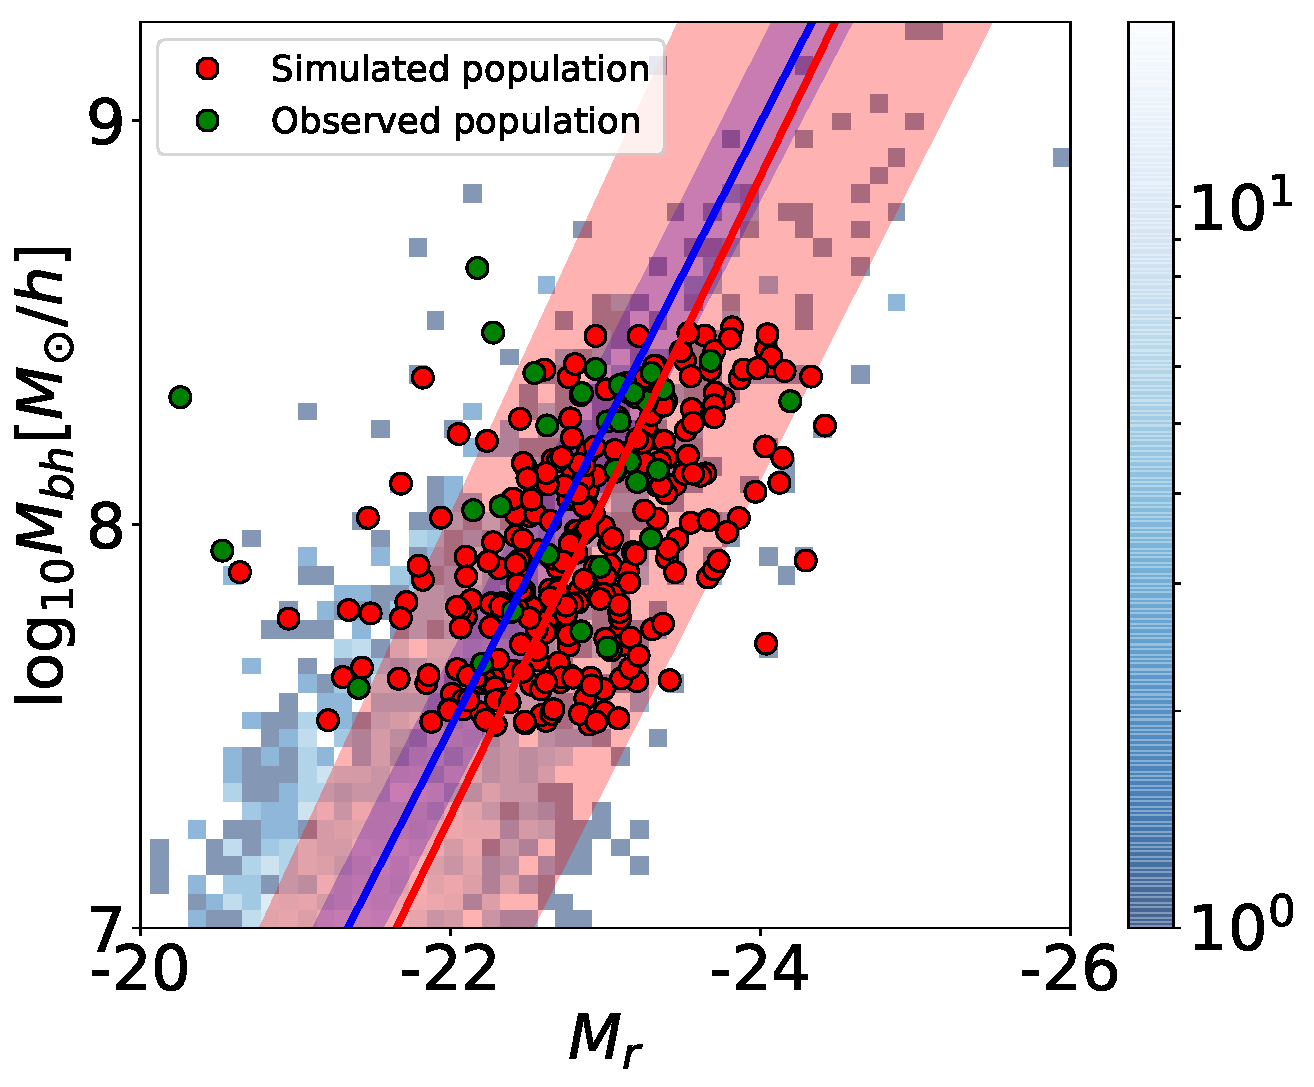
\includegraphics[width=0.5\linewidth]{MBII_ML.pdf} &
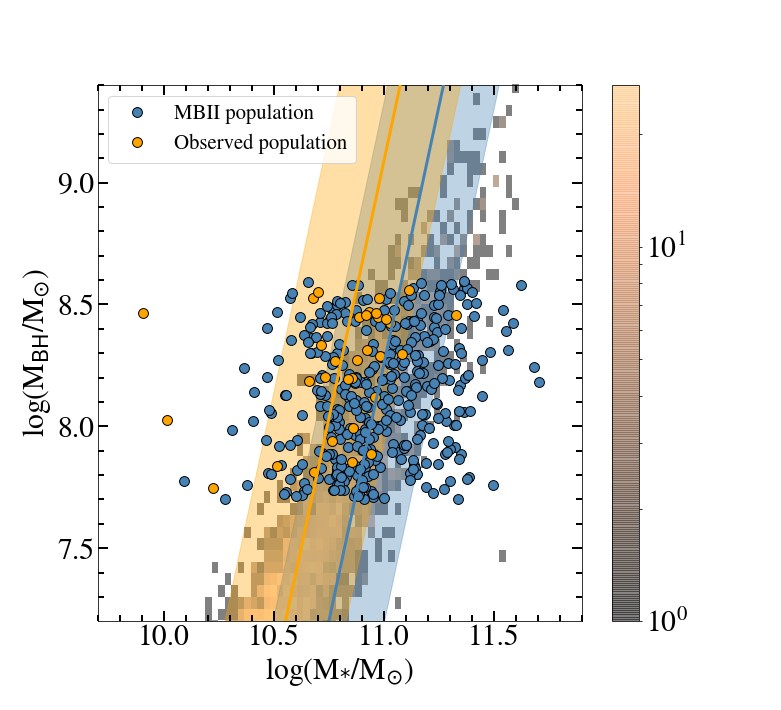
\includegraphics[width=0.5\linewidth]{MBII_MM.pdf} \\
\end{tabular}
\caption{
Comparing the scaling relations between the observed scaling relations to the predicted samples by the MBII simulation. In the left and right panel, we present the \mbh-\mr\ and \mbh-\mstar\ correlation, respectively. The blue grids are the overall galaxies that predicted in the MBII simulation and the red ones are selection effect considered. We red line shows the best-fit linear relations for the simulated selected sample. We fix the slope value to fit for the observed sample and find that the mismatch of the interceptions are within $1-\sigma$ difference for both relations. %{\bf For the right panel, I currently adopt a 3 Gyrs template for the HST sample...}
}
\label{fig:MBII_comp}
\end{figure*}

The comparisons between the observed scaling relations to the SAM model are presented in Figure~\ref{fig:SAM_comp}. Rather than predict each individual simulated sample, the SAM model describes the possibility clouds to demonstrate the density distribution of the scaling relations. We use two sets of color contours to demonstrate the possibility distribution at $z=1.5$ epoch, before and after adopting the selection window. The comparisons show great consistency that the hot zones in the SAM {\it selection-effect-considered} contours at $\log($\mbh$)~\in[7.5, 8.56]$ are well matched to the observed relations. We do not estimate the scatter for SAM model, but visually see that the observed relations are mostly located on top of the hot cloud, showing that the observed scatter should not be larger than the model one.

\begin{figure*}[t]%[!b]
\begin{tabular}{c c}
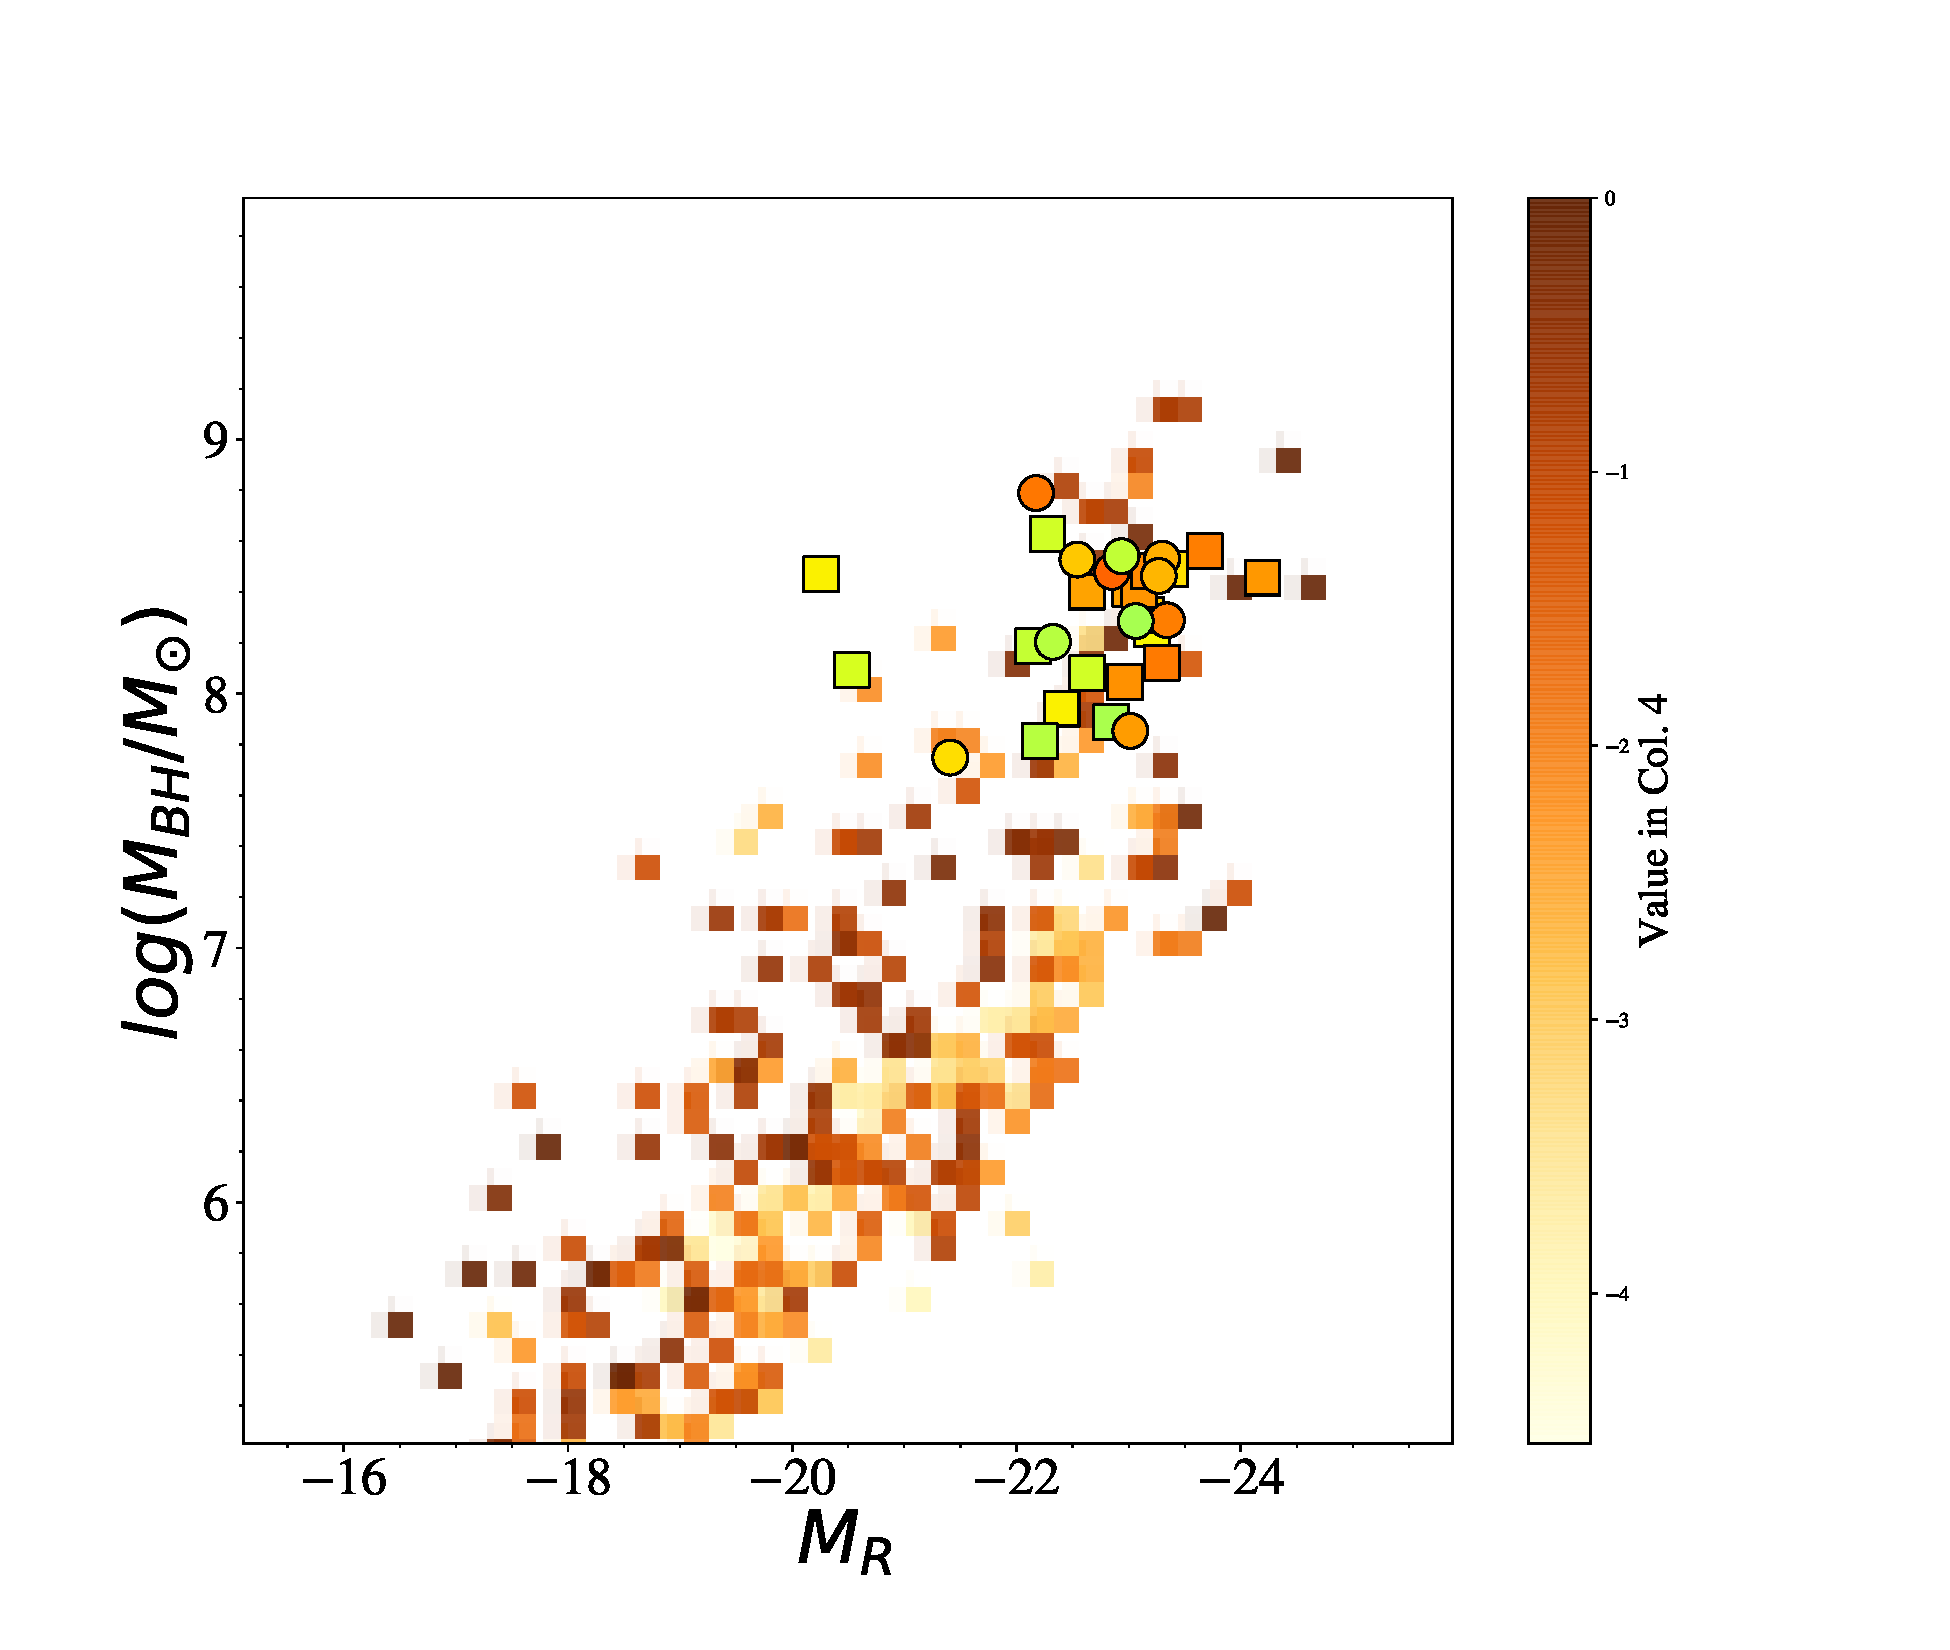
\includegraphics[trim = 0mm 0mm 26mm 0mm, clip, width=0.45\linewidth]{SAM_ML.pdf} &
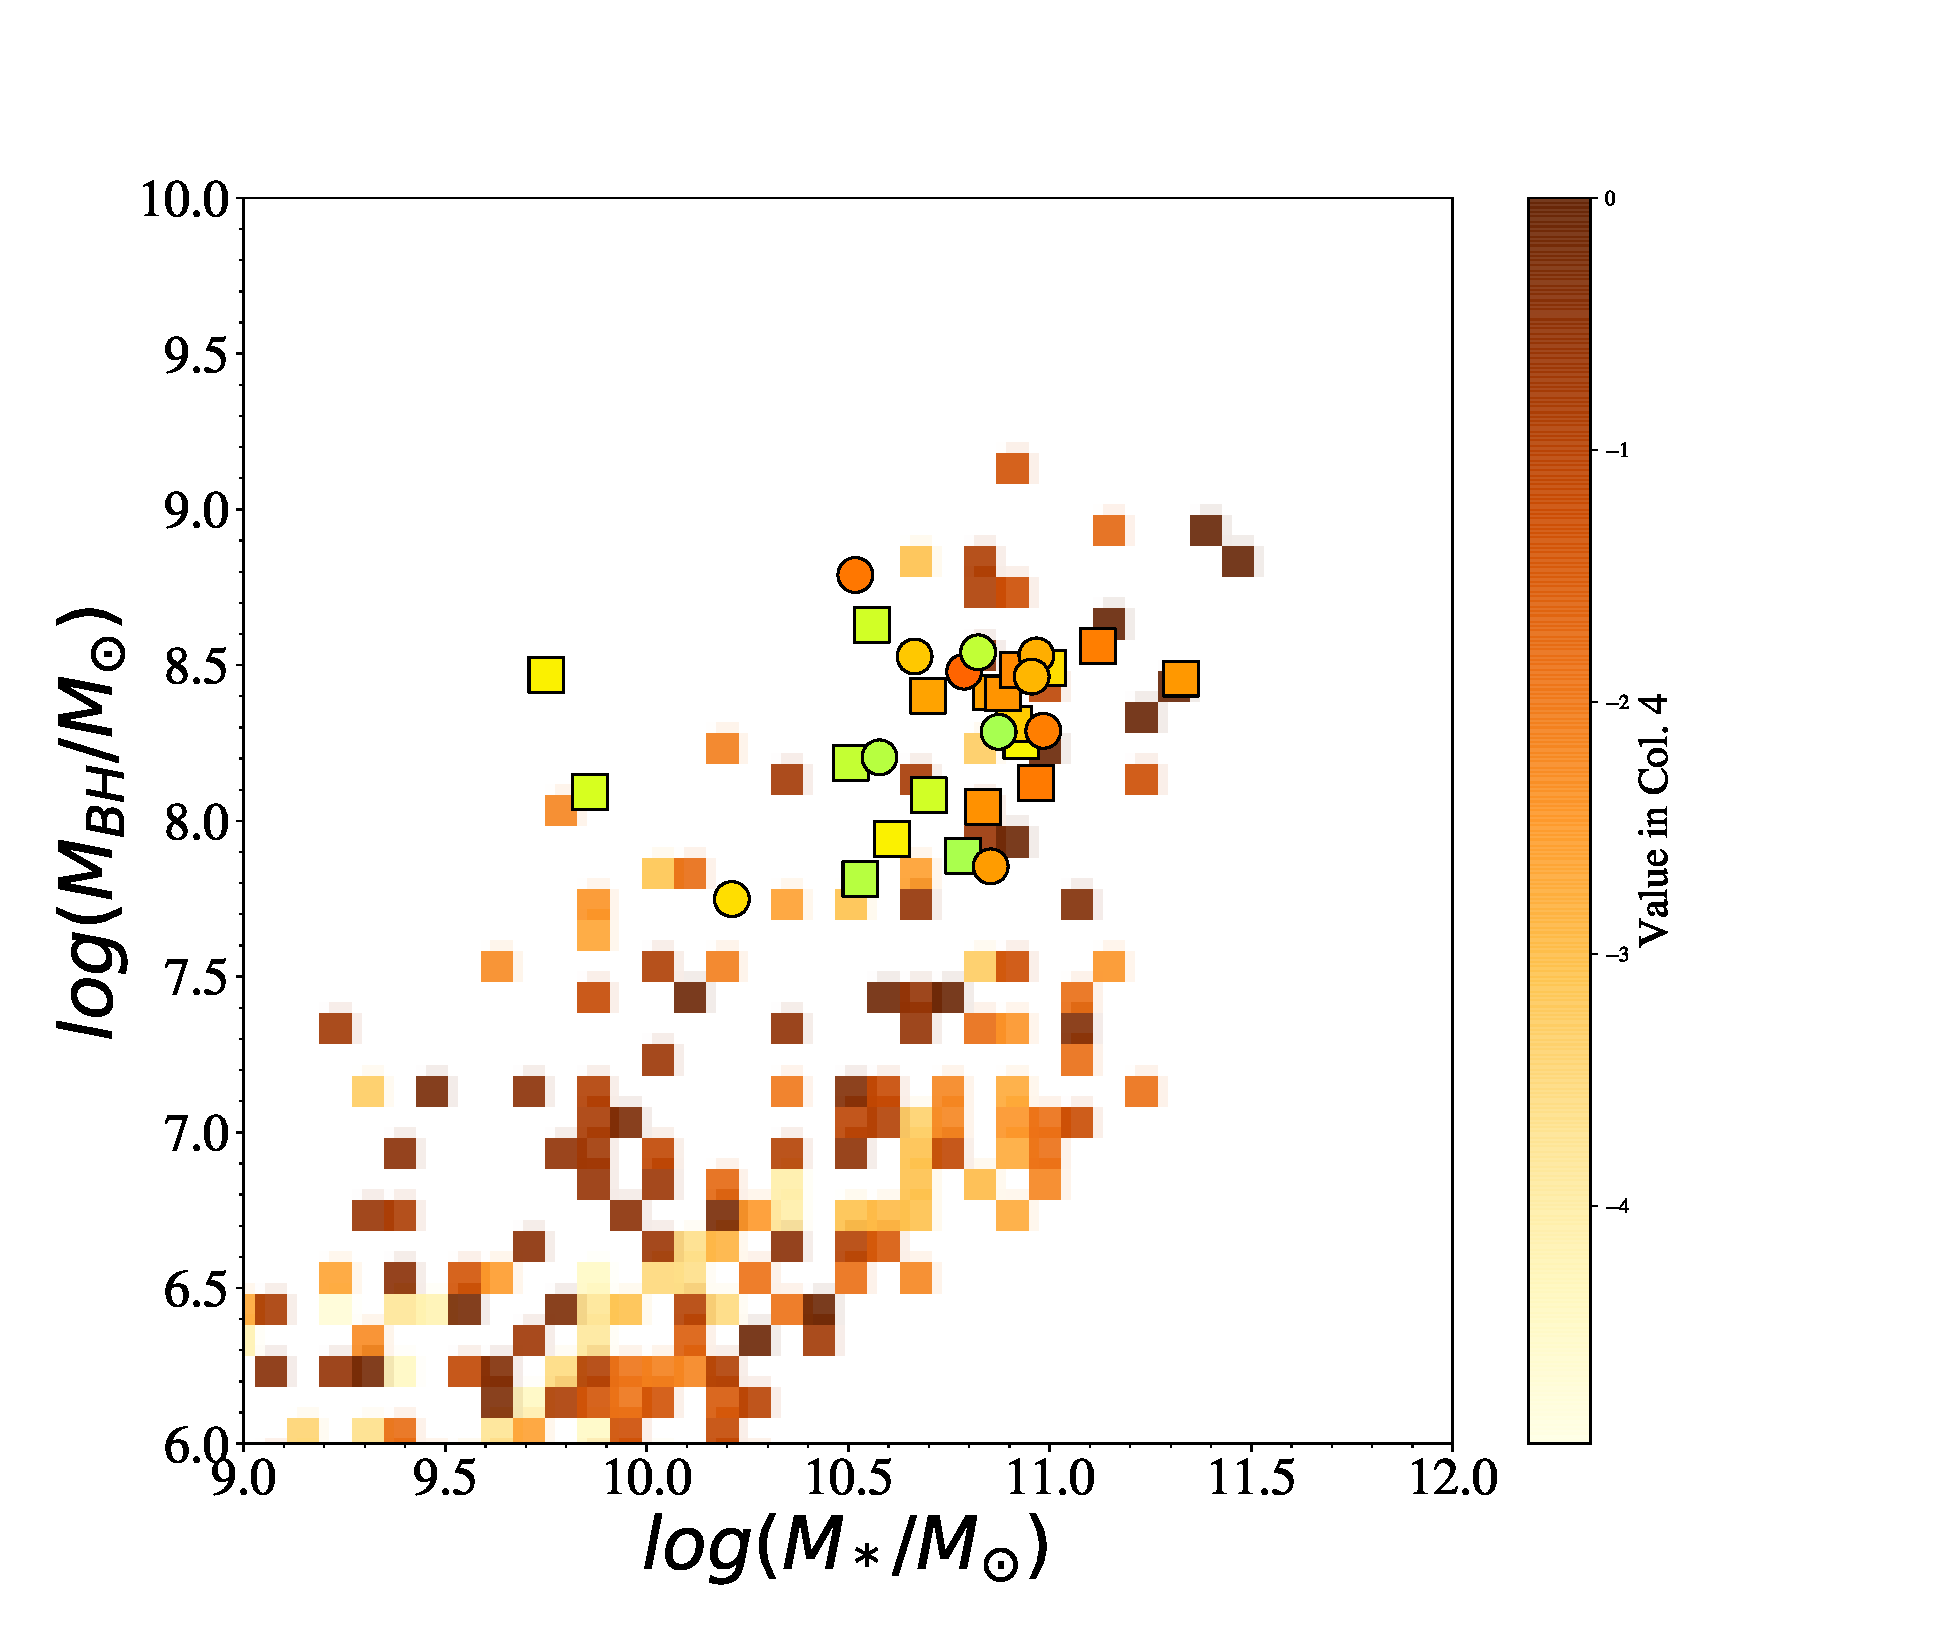
\includegraphics[trim = 24mm 0mm 0mm 0mm, clip, width=0.45\linewidth]{SAM_MMstar.pdf} \\
\end{tabular}
\caption{ Similar to the Figure~\ref{fig:MBII_comp}, we compare the observation to the SAM models. The blue background contours show the overall sample distribution and the red ones are the relations after considering the selecting effect. We see that the yellow contours are well matched to the hot zones for the red contours.
}
\label{fig:SAM_comp}
\end{figure*}

To help understand if any unexpected selection effects exist, we compare the distribution of the host-total flux ratio among these three samples. For the observed sample, we calculate the flux ratio at the imaging band, i.e., \hst/WFC3. For the simulated sample, we consider the AGN bolometric correction~\cite{Elvis1994} to estimate the AGN light flux at WFC3/F125W band. We compare their host-total flux histogram distribution in Figure~\ref{fig:comp_hist} and see that the three samples are well matched each other. The median values for the flux ratio distribution of the observed, MBII, SAM sample are $37.3\%$, $32.3\%$, and $42.8\%$, respectively. We perform the Kolmogorov-Smirnov test the inferred p-values are 0.34 (for observed -- MBII) and 0.14 (for observed -- SAM), respectively. {\bf Xuheng: more interpretations needs to put here}.

\begin{figure}[t]
\includegraphics[width=0.9\linewidth]{comp_host_ratio.pdf}
\caption{The comparison histogram of the host ratios among three referred samples, with median value indicated. The same selection effect are considered.
}
\label{fig:comp_hist}
\end{figure}

Without any physical mechanisms, the central limit theorem assumes that the scaling relations are the results by the random merger from a stochastic cloud at higher redshift. In this scenario, the scatter of the scaling relations has to be larger at higher redshift. However, the observed scatter of our high-$z$ sample do not present this feature. In fact, the obtained intrinsic scatter is only $\sim0.13$~dex, which is no more than the typical scatter at local relations in the literature ($\sim0.35$~dex)~\cite{Kormendy13, Gul++09}. Of course, the intrinsic scatter of our high-$z$ sample could be underestimated, since manually selected sample avoids the spreading of the properties and decrease the value of the scatter. Also, the observed \mbh\ are estimated using the robust \halpha\ line, which could have lower uncertainties level than expected (i.e., $\Delta$\mbh$<0.4$~dex), result in an overestimating of the error-budget and thus underestimating of intrinsic scatter. Still, even we do not take the uncertainties into account to calculate the scatter, the obtained value is $0.25$~dex, which is not larger than the local relations. Thus, the evidence of the low scatter in our measurements is likely to be true, which is against the central limit theorem and suggests that the physical mechanisms between the SMBH and its host galaxy are likely to exist. 

Between the MBII and SAM models, they all demonstrate an excellent agreement to the observed data; however, they adopted very different assumptions, recipes, and initial conditions. From another perspective to understand this agreement, there has to be a causal link between SMBH and its host galaxy to generate an ordering during their evolution, so that more massive BHs are linked to more massive galaxies with some intrinsic scatter. Once the selection function is well defined, the tight correlations would show up along with the selected sample.

Limited by the observations and the fact they are in good agreements to MBII and SAM, one can not rule out one simulating model from the other. Of course, there are differences between two simulating models. For example, the SAM sample trends to have more scatter than the MBII, especially before applying any selection function. More scatter could arise in SAM because the black hole feeding in this model is merger driven and so there is more stochasticities. In particular, the SAM cloud extends to the high \mbh\ with low stellar mass, which may not exist. These objects are usually with low Eddington ratio; thus an extension of this study to this region would be useful to discriminate between models.

Extending the redshift range of this study would also be very beneficial, giving that the scaling relation in the simulations shows different evolution at the different stage of the Universe. For higher redshift, the {\it James Webb Space Telescope} may provide high-quality imaging data of AGNs at redshift up to $z\sim7$. In the low redshift Universe, wide-area surveys with Subaru/HSC, LSST, and WFIRST offer much promise to build samples for studying these mass ratios and dependencies on other factors (e.g., environment).

%\textcolor{blue}{The details of the results could be presented.\\
%0. Compare the color of the sample?\\
%1. 2D KS test? \\
%2. More insightful inference from the comparing?
%}

%Discuss the result, What does this mean?

% \textcolor{blue}{If the final results show such feature:}
%The result also shows that the \mbh-\mstar\ relation has less scatter than the \mbh-\lhost\ relation, suggesting that the BH relation with \mstar\ are more fundamental than \lhost.
%This successful experience leads one conjecture that the other prediction by the simulations could likely to be right. For example, regarding the stellar components of galaxy which is the origin that related to the growth of BH, it is likely that the bulge masses are tightly related.

%\section*{Discussion}
%Some discussions should be placed in this section.
%On the observation side:\\
%0. The inferred host flux ratio by SED decomposition is consistent to the 2-D image decomposition, indicating the fidelity of these approaches?\\
%1. HST seems to reach its higher limit. In the future, the JWST is very promising to realize the evolution scenario at even higher redshift.\\
%On the simulation side:
%\\0. Introduce some the other 
%\\1. How do we discuss the role of AGN feedback?.

\begin{center}
{\bf \Large \uppercase{Methods} }
\end{center}

%\textbf{Observation data.} Our 32 new AGN systems are selected from four X-ray coverage fields including COSMOS (Civano et al. 2016), (E)- CDFS-S (Lehmer et al. 2005; Xue et al. 2011), and SXDS (Ueda et al. 2008) at redshift range $1.2<z<1.7$. The X-ray selected sample have low nuclear-to-host ratios, which facilitates the extraction of the host properties. We adopt the \hst/WFC3 infrared channel to derive the high spatial resolution imaging data, to carry out the decomposition of the AGN-host using two-dimensional flux distribution. The details of the \hst\ observation and the study are presented in the companion paper. Moreover, 21/32 systems have \hst/ACS band, together with some other ground-based observations, which would provide the host information in the other bands. In the next section, we infer the reliable K-correction for the rest-frame R band luminosity and the SED to infer the stellar mass. The \mbh\ of our sample have been estimated by \halpha\ and \hbeta\ in the FMOS survey. Comparing to the \Mgii\ and \Civ, the \mbh\ by broad Balmer lines are more trustworthy. The estimated value of the \mbh\ are listed in the companion paper.
%\textcolor{blue}{Do we need to list the \mbh\ and host properties in a table in this paper?}

\textbf{Imaging data, decomposition and inference of host properties.} 
%1. Imaging data. 2. Inferring host light. 3. Color inference. Rest frame R band and stellar mass.
We adopted the \hst/WFC3 infrared channel and selected to use the filters F125W $(1.2<z<1.44)$ and F140W $(1.44<z<1.7)$ according to the redshift of the targets, to observe the imaging data for the 32 AGN systems through the \hst\ program GO-15115 (PI: John Silverman). We obtain six dither exposures with total exposure time $\sim2394s$ and using  {\sc astrodrizzle} software package to co-add the final image with pixel scale as 0\farcs0642. To mitigate the contamination from both the sky and the detector, we adopt the {\sc photuils} tools to estimate and remove them accurately.

To address the bias which might be raised by the unknown PSF, we manually collect the isolated-unsaturated PSF-stars from the 32 observed fields, to assemble a PSF library for the fitting. To decompose each AGN image, we assume the unresolved active nuclei as the scaled point source and the host galaxy as the \sersic\ profile. We adopt imaging modeling tool \lenstronomy\cite{lenstronomy} to simultaneously fit their 2-D flux distribution, taking each PSF one by one from the library. Based on the reduced $\chi^2$, we are capable of evaluating the performance of each PSF. We adopt the result from the top-eight PSFs and infer the host property, including flux, \reff, \sersic\ index, using a weighted arithmetic mean.

21/32 images in the COSMOS survey also have imaging data in the ACS/F814W with drizzled pixel scale as 0\farcs03, providing us the multi-band information. We decompose the AGN image in the ACS band to obtain the color of the host. We find that the 1Gyr template would well match their color from which we estimate the rest-frame R band luminosity and stellar mass. A Salpeter initial mass function is employed consistently to the observed and simulated sample.

%\textbf{SED fitting and host properties}
%We perform the SED fitting to derive the robust physical properties of the host galaxy, including the rest-frame R band luminosity and stellar mass. 
%21/32 AGN systems have rest-frame UV imaging data by \hst-ACS/F814W\cite{Scoville2007}. We perform the same approach to decompose the photometry of the host light at UV. Since the host inference by IR band is superior to the one by UV band, while fitting UV image, we fix the \reff\ and \sersic\ index as the value inferred by \hst/WFC3 to derive the host flux.
%We furthermore combine the \hst\ inference to the ground-based AGN photometry to carry out the SED fitting. \textcolor{blue}{Details and the figures need to be presented.}
%Adopting the best fit SED stellar template to the \hst/WFC3 flux, we derive the \lhost${,_R}$ and \mstar.


\textbf{Simulations.} 
Describe the approaches used in the simulation.

%%%%%%%%%%%%%%%%%%%%%%%%%%%%%%%%%%%%%%%%%%%%%%%%%%%%%%%%%%%%%%%%%%%%%%%%%%%%%%%

\section*{References}
\bibliography{references} 


\begin{addendum}
 \item[Acknowledgements] 
%X. Ding acknowledges support by China Postdoctoral Science Foundation Funded Project (No. 2017M622501).

%
\item[Correspondence] %Correspondence and requests for materials should be addressed to Xuheng Ding ~(email:dxh@astro.ucla.edu).
\item[Author Contributions] xxx measure xxx, xxx extract the simulation from xx.
\end{addendum}

%%%%%%%%%%%%%%%%%%%%%%%%%%%%%%%%%%%%%%%%%%%%%%%%%%%%%%%%%%%%%%%%%%%%%%%%%%%%%%%
\section*{Additional information}
\textbf{Code availability.} The \lenstronomy, which is used to decompose the AGN image  
%The data reduction package used to process the SAMI data is available at http://ascl.net/1407.006, and makes use of 2dfdr: http://www.aao.gov.au/science/software/2dfdr. To derive the stellar kinematic parameters and the lick absorption line strengths, we use the publicly available penalised pixel-fitting (pPXF) code from M. Capppellari: {http://www-astro.physics.ox.ac.uk/~mxc/software/\#ppxf}. For the adaptive LOESS smoothing, we use the code from M. Cappellari obtained from: http://www-astro.physics.ox.ac.uk/~mxc/software/\#loess

\textbf{Data availability.} All the inference of the AGN properties are presented in the companion paper.
%All reduced data-cubes in the GAMA fields used in this Letter are available on: http://datacentral.aao.gov.au/asvo/surveys/sami/, as part of the first SAMI Galaxy Survey data release. Stellar kinematic data products will become available in the second SAMI Galaxy Survey data release. 


%%%%%%%%%%%%%%%%%%%%%%%%%%%%%%%%%%%%%%%%%%%%%%%%%%%%%%%%%%%%%%%%%%%%%%%%%%%%%%%


%\clearpage
%\newpage
%\onecolumn
%\begin{center}
%{\bf \Large \uppercase{Supplementary information} }
%\end{center}
%
%\setcounter{figure}{0}
%\vspace{2cm}
%
%\begin{figure}[!h]
%\begin{center}
%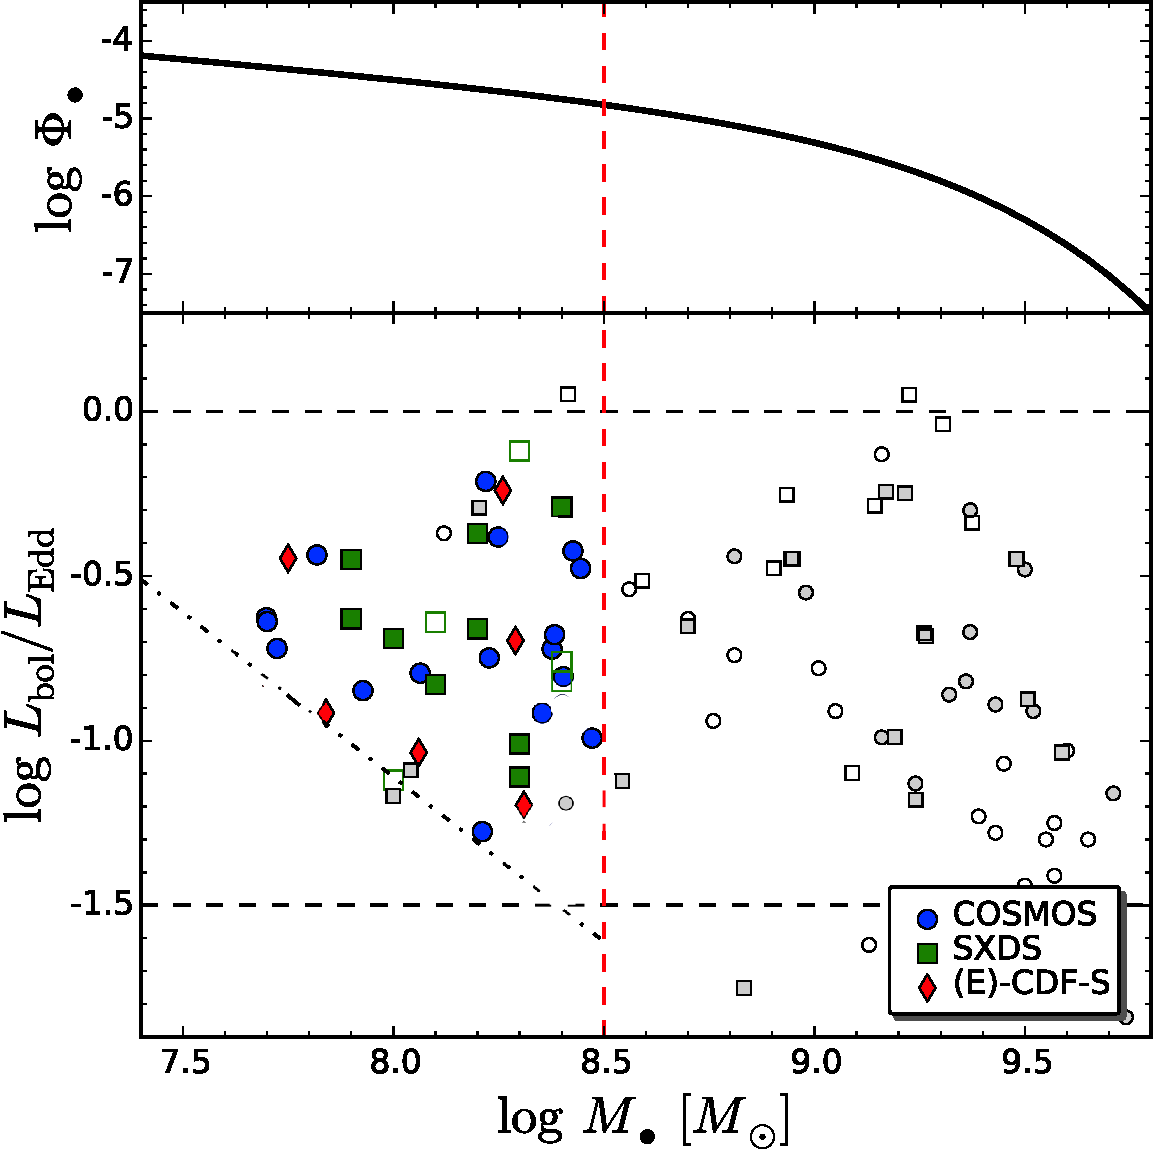
\includegraphics[width=0.8\linewidth]{hst_sample_bhmf.pdf}
%\caption{
%The selection function of our observation data. Eddington ratios (LBol/LEdd) and BH masses (bottom panel) of our sample (in color) that fall well-below the knee of the BH mass function at z = 1.5 (top panel; Schulze et al. 2015). Dashed lines (vertical and horizontal) denote our selection window with the slanted line only shown to approximately illustrate the effect of a luminosity limit, inherent in the parent catalogs. For reference, we indicate the high-z luminous SDSS QSO samples (grey squares - Peng et al. 2006; grey circles - Decarli et al. 2010) with all falling above our chosen upper mass limit.
%}
%\label{fig:support}
%\end{center}
%\end{figure}

\end{document}
